\documentclass[11pt,letterpaper]{article}
\usepackage[lmargin=1in,rmargin=1in,tmargin=1in,bmargin=1in]{geometry}
\usepackage{../style/homework}
\setbool{quotetype}{true} % True: Side; False: Under
\setbool{hideans}{false} % Student: True; Instructor: False

% -------------------
% Content
% -------------------
\begin{document}

\homework{1: Due 01/24}{When I was young I observed that nine out of every ten things I did were fails, so I did ten times more work.}{George Bernard Shaw}

% Problem 1
\problem{10} A certain subspecies of oak tree grows to an average height of 87~ft. After five years of growth, the growth rate of these oaks is approximately constant at a rate of 13~in per year. An ecologist finds the current height of an oak estimated to be 8~years in age to be 8~ft tall. Let $H(t)$ denote the height (in feet) of the tree $t$ years from its `birth.' 
	\begin{enumerate}[(a)]
	\item Explain why $H(t)$ is approximately linear. 
	\item Find $H(t)$ and sketch it in the plot below. 
	\item Interpret the slope of $H(t)$.
	\item Interpret the $y$-intercept for $H(t)$.
	\item Find approximately how many more years until the tree reaches its `adult height.' 
	\end{enumerate} 

\sol 
\begin{enumerate}[(a)]
\item We know that the growth rate of oaks after 5~years of growth is approximately constant. Functions with a constant rate of change are linear. Therefore, it must be that $H(t)$ is approximately linear (after the first 5~years of growth). 

\item We know from (a) that $H(t)$ is approximately linear. Therefore, after the first 5~years of growth, $H(t)= mt + b$. Because these oaks grow an average of 13~in per year ($\frac{13}{12}= 1.08333$~ft per year), we know that $m= 1.08333$. Because the tree is 8~ft tall after 8~years from its `birth', we know that $H(8)= 8$. But we have $8= H(t)= 1.08333(8) + b= 8.66664 + b$. This implies that $b= 8 - 8.66664= -0.66664$. Therefore, $H(t)= 1.08333t - 0.66664$. 

\item We know that $m > 0$, so that $H(t)$ must be increasing. As $m= 1.08333= \frac{\Delta H}{\Delta t}$, the tree grows by approximately 1.08333~feet per year. 

\item The $y$-intercept of $H(t)$ is $b= -0.66664$. We know that $b= H(0)$, i.e. the height of the tree at $t= 0$---its birth. But height cannot be negative. Therefore, $b$ has no interpretation in the context of the problem. 

\item The average adult height for this tree is 87~ft. We want a time $t_0$ such that $H(t_0)= 87$. But then we have $87= 1.08333t_0 - 0.66664$, which implies $1.08333t_0= 87.6666$. Therefore, $t_0\approx 80.92$~years. But this is the years from `birth' to reach this height. Therefore, the tree should reach its adult height in approximately $80.92 - 8= 72.92$~years from now. 
\end{enumerate}
	
	\vfill
	
	\[
	\fbox{
	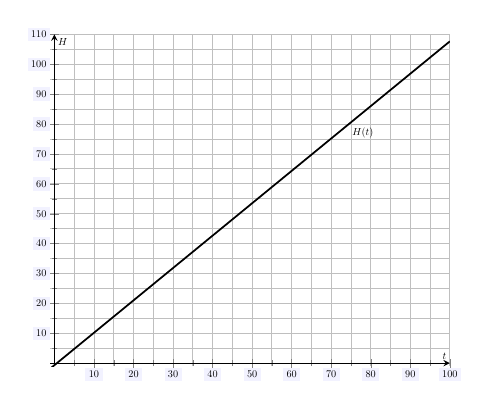
\begin{tikzpicture}[scale=0.74,every node/.style={scale=0.5}]
	\begin{axis}[
	grid=both,
	axis lines=middle,
	ticklabel style={fill=blue!5!white},
	xmin= -1, xmax=100,
	ymin= -1, ymax=110,
	xtick={0,10,...,100},
	ytick={0,10,...,110},
	minor x tick num = 1,
	minor y tick num = 1,
	xlabel=\(t\),ylabel=\(H\),
	]
	\addplot[line width=0.03cm,domain= -1:100] ({x},{1.08333*x - 0.66664});
	\node at (78,77) {$H(t)$};
	\end{axis}
	\end{tikzpicture}
	}
	\] 



\newpage



% Problem 2
\problem{10} Compute the following:
	\begin{enumerate}[(a)]
	\item 76\% of 8,571
	\item 16\% of 56.8
	\item 155\% of 11
	\item 78 decreased by 54\%
	\item 280 increased by 40\%
	\item 54 increased by 110\%
	\end{enumerate} \pspace

\sol 
\begin{enumerate}[(a)]
\item 
	\[
	\text{76\% of 8,571}= 8,\!571(0.76)= 6,\!513.96
	\] \pspace

\item 
	\[
	\text{16\% of 56.8}= 56.8(0.16)= 9.088
	\] \pspace

\item 
	\[
	\text{155\% of 11}= 11(1.55)= 17.05
	\] \pspace

\item 
	\[
	\text{78 decreased by 54\%}= 78 (1 - 0.54)= 78(0.46)= 35.88
	\] \pspace

\item 
	\[
	\text{280 increased by 40\%}= 280 (1 + 0.40)= 280(1.40)= 392
	\] \pspace

\item 
	\[
	\text{54 increased by 110\%}= 54 (1 + 1.10)= 54(2.1)= 113.4
	\]
\end{enumerate}
	
	

\newpage



% Problem 3
\problem{10} The economy in a certain nation is devolving into panic due to recent world events. Economists in the country are trying to keep track of the resulting inflation. A good which currently costs \$30 is estimated to increase in price by 8\% each month over the next 2 months. 
	\begin{enumerate}[(a)]
	\item How much will the good cost after the end of the two months? Be sure to justify your answer. 
	\item Is your answer in (a) the same as raising the original price by 16\%? Explain. 
	\item If the price simply increased to \$40, by what percentage did the price increase from the original price?
	\item If the inflation continues at this rate, how much will the good cost two years from now?	
	\end{enumerate} \pspace

\sol 
\begin{enumerate}[(a)]
\item If we want to compute $N$ repeatedly increased or decreased by a \% a total of $n$ times, we compute $N(1 \pm \%_d)^n$, where $\%_d$ is the percentage written as a decimal, and we choose `$+$' if it is a repeated percentage increase and `$-$' if it is a repeated percentage decrease. But then if the price of a good, $P= \$30$, increased by 8\% every month for 2~months, the final price would be\dots
	\[
	\$30 (1 + 0.08)^2= \$30(1.08)^2= \$30(1.1664) \approx \$34.99
	\]
Therefore, if the inflation rate continues to be 8\% across the next two months, the good will cost \$34.99. \pspace

\item If we want to compute $N$ increased or decreased by a \%, we compute $N \cdot (1 \pm \%_d)$, where $\%_d$ is the percentage written as a decimal and we choose `$+$' if it is a percentage increase and choose `$-$' if it is a percentage decrease. Increasing \$30 by 16\%, we have $\$30(1 + 0.16)= \$30(1.16)= \$34.80$. This is not the same as in (a). This is because percentages are multiplicative---not additive. \pspace

\item This is\dots
	\[
	\text{Percentage Change}= \dfrac{\text{New Price} - \text{Original Price}}{\text{Original Price}} \cdot 100= \dfrac{\$40 - \$30}{\$30} \cdot 100= \dfrac{\$10}{\$30} \cdot 100= 33.33\%
	\] \pspace

\item After two years, i.e. 24~months, with the good increasing in price by 8\% each month, the good will cost\dots
	\[
	\$30 (1 + 0.08)^{24}= \$30(1.08)^{24}= \$30(6.34118) \approx \$190.24
	\]
\end{enumerate}


\end{document}